\documentclass[11pt,a4paper]{article}

% Packages
\usepackage[british]{babel}
\usepackage[utf8]{inputenc}
\usepackage[T1]{fontenc}
\usepackage{geometry}
\geometry{a4paper, margin=2.5cm}
\usepackage{setspace}
\usepackage{graphicx}
\usepackage{booktabs}
\usepackage{tabularx}
\usepackage{xcolor}
\usepackage{tikz}
\usetikzlibrary{positioning, shapes, arrows}
\usepackage[breaklinks=true,hidelinks]{hyperref}

\definecolor{tier1}{RGB}{46, 125, 50}
\definecolor{tier2}{RGB}{251, 192, 45}
\definecolor{tier3}{RGB}{245, 124, 0}
\definecolor{tier4}{RGB}{211, 47, 47}

\title{\textbf{Metric Selection Guide:\\Black-Box Evaluation for Clinical LLMs}}
\author{Supplementary Document}
\date{November 2025}

\begin{document}

\maketitle
\onehalfspacing

\section{Executive Decision Matrix}

This document provides actionable guidance for selecting evaluation metrics based on your deployment constraints, computational budget, and regulatory requirements.

\section{The Fundamental Question}

\begin{center}
\fbox{\parbox{0.9\textwidth}{
\textbf{Critical Constraint}: Do you have access to model internals (weights, logits, activations)?

\begin{itemize}
    \item \textbf{NO} $\rightarrow$ You \textit{must} use black-box metrics (Tiers 1--3)
    \item \textbf{YES} $\rightarrow$ You \textit{may} use white-box metrics (Tier 4), but black-box is still recommended for portability
\end{itemize}
}}
\end{center}

\section{Metric Decision Tree}

\begin{figure}[h]
\centering
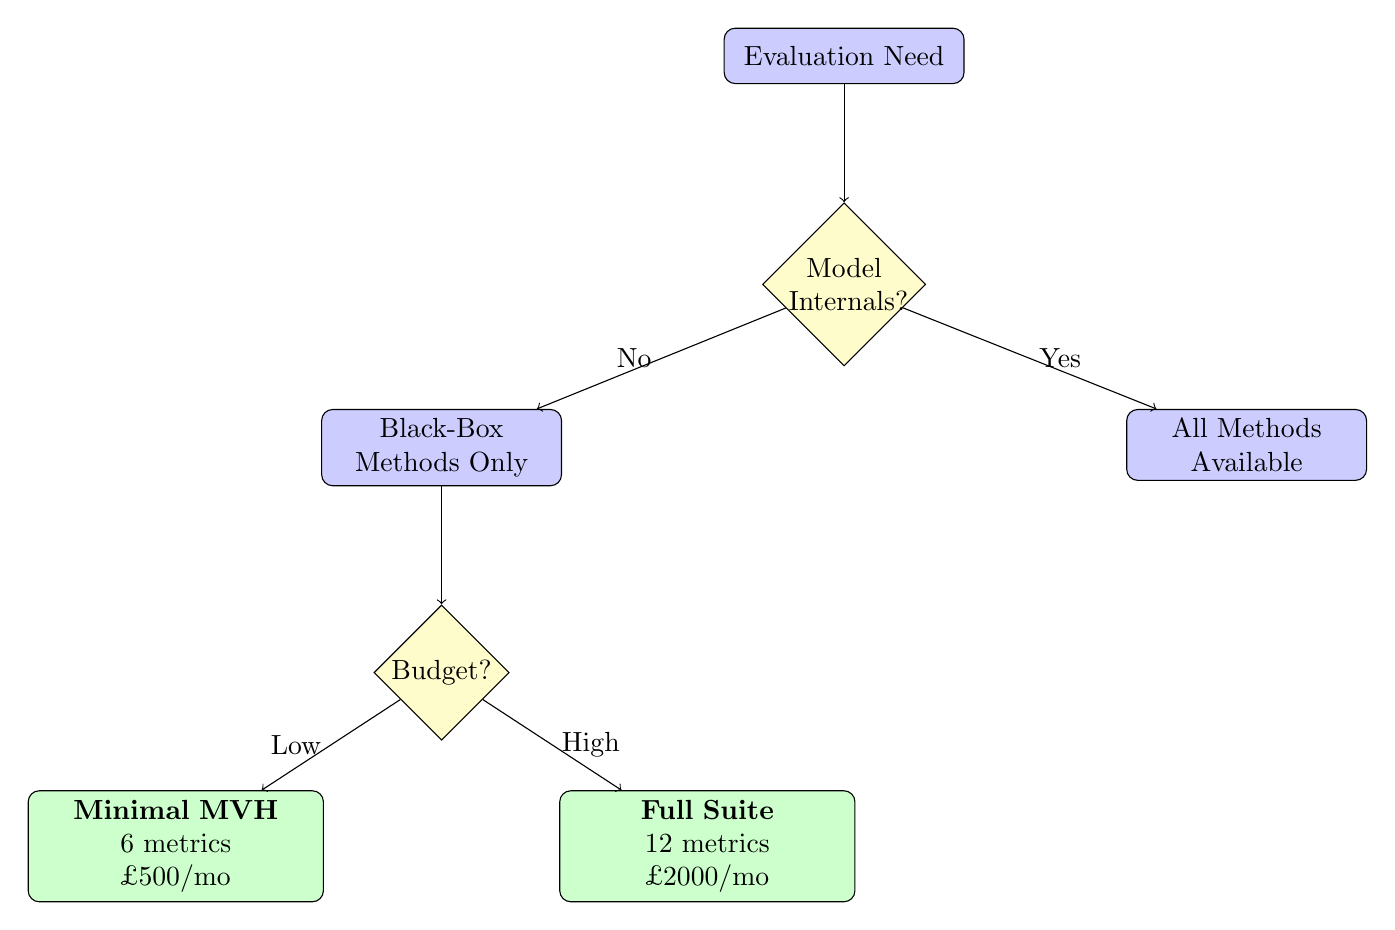
\begin{tikzpicture}[
    node distance=1.5cm,
    decision/.style={diamond, draw, fill=yellow!20, text width=4em, text centered, inner sep=0pt, minimum height=3em},
    block/.style={rectangle, draw, fill=blue!20, text width=8em, text centered, rounded corners, minimum height=2em},
    endpoint/.style={rectangle, draw, fill=green!20, text width=10em, text centered, rounded corners, minimum height=2em}
]

\node [block] (start) {Evaluation Need};
\node [decision, below=of start] (access) {Model\\ Internals?};
\node [block, below left=of access, xshift=-2cm] (blackbox) {Black-Box\\ Methods Only};
\node [block, below right=of access, xshift=2cm] (whitebox) {All Methods\\ Available};
\node [decision, below=of blackbox] (budget) {Budget?};
\node [endpoint, below left=of budget] (minimal) {\textbf{Minimal MVH}\\ 6 metrics\\ £500/mo};
\node [endpoint, below right=of budget] (full) {\textbf{Full Suite}\\ 12 metrics\\ £2000/mo};

\draw [->] (start) -- (access);
\draw [->] (access) -- node[left] {No} (blackbox);
\draw [->] (access) -- node[right] {Yes} (whitebox);
\draw [->] (blackbox) -- (budget);
\draw [->] (budget) -- node[left] {Low} (minimal);
\draw [->] (budget) -- node[right] {High} (full);

\end{tikzpicture}
\caption{Metric Selection Decision Tree}
\end{figure}

\section{Detailed Metric Scorecards}

\subsection{Scoring Dimensions}

Each metric is scored on five dimensions (1--5 scale, 5 = best):

\begin{itemize}
    \item \textbf{Black-Box}: Works without model internals
    \item \textbf{Ease}: Implementation complexity
    \item \textbf{Clinical}: Interpretability for clinicians/regulators
    \item \textbf{Compute}: Resource efficiency
    \item \textbf{Signal}: Diagnostic power
\end{itemize}

\subsection{Study A: Faithfulness Metrics}

\begin{table}[H]
\centering
\caption{Study A Metric Scorecards}
\begin{tabular}{@{}lccccccc@{}}
\toprule
\textbf{Metric} & \textbf{Black-Box} & \textbf{Ease} & \textbf{Clinical} & \textbf{Compute} & \textbf{Signal} & \textbf{Total} & \textbf{Rank} \\
\midrule
$\Delta_{\text{Reasoning}}$ & 5 & 5 & 5 & 4 & 5 & 24/25 & \textcolor{tier1}{\#1} \\
Step-F1 & 5 & 4 & 4 & 5 & 4 & 22/25 & \textcolor{tier2}{\#2} \\
$R_{SB}$ & 5 & 4 & 3 & 5 & 3 & 20/25 & \textcolor{tier3}{\#3} \\
CC-SHAP & 1 & 1 & 2 & 1 & 5 & 10/25 & \textcolor{tier4}{\#4} \\
\bottomrule
\end{tabular}
\end{table}

\textbf{Recommendation}: Deploy $\Delta_{\text{Reasoning}}$ as primary gate. Add Step-F1 if you have gold reasoning traces (OpenR1-Psy). Use $R_{SB}$ only for adversarial bias testing.

\subsection{Study B: Sycophancy Metrics}

\begin{table}[H]
\centering
\caption{Study B Metric Scorecards}
\begin{tabular}{@{}lccccccc@{}}
\toprule
\textbf{Metric} & \textbf{Black-Box} & \textbf{Ease} & \textbf{Clinical} & \textbf{Compute} & \textbf{Signal} & \textbf{Total} & \textbf{Rank} \\
\midrule
$P_{\text{Syc}}$ & 5 & 5 & 5 & 5 & 5 & 25/25 & \textcolor{tier1}{\#1} \\
Flip Rate & 5 & 5 & 5 & 5 & 4 & 24/25 & \textcolor{tier1}{\#2} \\
$H_{Ev}$ & 5 & 3 & 4 & 3 & 5 & 20/25 & \textcolor{tier2}{\#3} \\
ToF & 5 & 5 & 5 & 4 & 3 & 22/25 & \textcolor{tier2}{\#4} \\
TDR & 5 & 4 & 3 & 4 & 3 & 19/25 & \textcolor{tier3}{\#5} \\
SSM & 5 & 4 & 2 & 5 & 3 & 19/25 & \textcolor{tier3}{\#6} \\
$\Delta_{\text{latent}}$ & 1 & 2 & 2 & 3 & 5 & 13/25 & \textcolor{tier4}{\#7} \\
\bottomrule
\end{tabular}
\end{table}

\textbf{Recommendation}: Deploy $P_{\text{Syc}}$ + Flip Rate as core sycophancy suite. Add $H_{Ev}$ if hallucination detection is critical. ToF is excellent for multi-turn safety windows.

\subsection{Study C: Longitudinal Drift Metrics}

\begin{table}[H]
\centering
\caption{Study C Metric Scorecards}
\begin{tabular}{@{}lccccccc@{}}
\toprule
\textbf{Metric} & \textbf{Black-Box} & \textbf{Ease} & \textbf{Clinical} & \textbf{Compute} & \textbf{Signal} & \textbf{Total} & \textbf{Rank} \\
\midrule
Entity Recall & 5 & 4 & 5 & 4 & 5 & 23/25 & \textcolor{tier1}{\#1} \\
ToF & 5 & 5 & 5 & 5 & 3 & 23/25 & \textcolor{tier1}{\#2} \\
$K_{\text{Conflict}}$ & 5 & 3 & 4 & 3 & 4 & 19/25 & \textcolor{tier2}{\#3} \\
Continuity Score & 5 & 3 & 3 & 4 & 3 & 18/25 & \textcolor{tier3}{\#4} \\
PDSQI-9 & 5 & 1 & 5 & 1 & 5 & 17/25 & \textcolor{tier3}{\#5} \\
\bottomrule
\end{tabular}
\end{table}

\textbf{Recommendation}: Deploy Entity Recall as primary drift indicator. ToF provides session length guidance. Add $K_{\text{Conflict}}$ for contradiction detection. Avoid PDSQI-9 unless you have £££ budget for LLM-as-Judge calls.

\section{The Minimal Viable Harness (MVH)}

\subsection{Configuration}

\begin{table}[H]
\centering
\caption{Minimal Viable Harness Specification}
\begin{tabularx}{\textwidth}{@{}lXc@{}}
\toprule
\textbf{Study} & \textbf{Metrics} & \textbf{Total LOC} \\
\midrule
Study A & $\Delta_{\text{Reasoning}}$ (Primary) + Step-F1 (Diagnostic) & 80 \\
Study B & $P_{\text{Syc}}$ (Primary) + Flip Rate (Diagnostic) & 40 \\
Study C & Entity Recall (Primary) + ToF (Diagnostic) & 50 \\
\midrule
\textbf{Total} & \textbf{6 metrics} & \textbf{170 lines} \\
\bottomrule
\end{tabularx}
\end{table}

\subsection{Cost Breakdown}

\begin{table}[H]
\centering
\caption{MVH Operational Costs (per month)}
\begin{tabularx}{\textwidth}{@{}lXr@{}}
\toprule
\textbf{Component} & \textbf{Description} & \textbf{Cost (GBP)} \\
\midrule
Model API Calls & 2 runs per vignette × 200 vignettes × 3 studies & £300 \\
scispaCy NER & Free (local) & £0 \\
DeBERTa NLI & Free (Hugging Face) & £0 \\
Compute (GPU) & Occasional fine-tuning / local inference & £100 \\
Storage & Logs, outputs, CSVs & £10 \\
Dashboard & Streamlit Community (free tier) & £0 \\
\midrule
\textbf{Total} & & \textbf{£410/mo} \\
\bottomrule
\end{tabularx}
\end{table}

\subsection{Deliverables}

\begin{itemize}
    \item \textbf{Clinical Safety Card}: Single-page PDF with 6 headline numbers
    \item \textbf{Per-Model Report}: Comparative table (PsyLLM vs Qwen vs GPT-OSS)
    \item \textbf{Failure Examples}: 10 qualitative examples per failure mode
    \item \textbf{Regulatory Brief}: 2-page executive summary for governance teams
\end{itemize}

\section{The Full Suite (Research/High-Assurance)}

\subsection{Configuration}

\begin{table}[H]
\centering
\caption{Full Suite Specification}
\begin{tabularx}{\textwidth}{@{}lXc@{}}
\toprule
\textbf{Study} & \textbf{Metrics} & \textbf{Total LOC} \\
\midrule
Study A & $\Delta_{\text{Reasoning}}$, Step-F1, $R_{SB}$ & 140 \\
Study B & $P_{\text{Syc}}$, Flip Rate, $H_{Ev}$, ToF, TDR, SSM & 180 \\
Study C & Entity Recall, ToF, $K_{\text{Conflict}}$, Continuity Score & 140 \\
\midrule
\textbf{Total} & \textbf{13 metrics} & \textbf{460 lines} \\
\bottomrule
\end{tabularx}
\end{table}

\subsection{Cost Breakdown}

\begin{table}[H]
\centering
\caption{Full Suite Operational Costs (per month)}
\begin{tabularx}{\textwidth}{@{}lXr@{}}
\toprule
\textbf{Component} & \textbf{Description} & \textbf{Cost (GBP)} \\
\midrule
Model API Calls & 5 runs per vignette × 300 vignettes × 3 studies & £1200 \\
NLI Model Calls & Evidence hallucination + conflict detection & £300 \\
Embedding Models & Continuity score (MiniLM) & £50 \\
Compute (GPU) & Local inference for baselines & £200 \\
Storage & Extended logs, multi-seed runs & £50 \\
Dashboard & Streamlit Pro + Grafana & £100 \\
\midrule
\textbf{Total} & & \textbf{£1900/mo} \\
\bottomrule
\end{tabularx}
\end{table}

\section{Tradeoff Analysis: Key Decisions}

\subsection{Decision 1: Gold Reasoning Traces (Step-F1)}

\begin{table}[H]
\centering
\begin{tabularx}{\textwidth}{@{}lXX@{}}
\toprule
& \textbf{With Step-F1} & \textbf{Without Step-F1} \\
\midrule
\textbf{Benefit} & Validates reasoning content quality against expert gold standards & Simpler implementation \\
\textbf{Cost} & Requires annotated dataset (OpenR1-Psy has 150--200 items) & Lose diagnostic insight \\
\textbf{Recommendation} & Use if dataset available & Skip for pilot phase \\
\bottomrule
\end{tabularx}
\end{table}

\subsection{Decision 2: Evidence Hallucination ($H_{Ev}$)}

\begin{table}[H]
\centering
\begin{tabularx}{\textwidth}{@{}lXX@{}}
\toprule
& \textbf{With $H_{Ev}$} & \textbf{Without $H_{Ev}$} \\
\midrule
\textbf{Benefit} & Catches malignant lying (fake symptoms) & Simpler sycophancy detection \\
\textbf{Cost} & Requires NLI model + claim extraction (80 LOC) & Cannot distinguish polite vs malignant \\
\textbf{Recommendation} & Critical for high-stakes clinical use & Skip for general chatbots \\
\bottomrule
\end{tabularx}
\end{table}

\subsection{Decision 3: Multi-Turn Simulation (ToF, TDR)}

\begin{table}[H]
\centering
\begin{tabularx}{\textwidth}{@{}lXX@{}}
\toprule
& \textbf{With Multi-Turn} & \textbf{Without Multi-Turn} \\
\midrule
\textbf{Benefit} & Defines safe conversation window (ToF). Measures decay speed (TDR) & Faster evaluation \\
\textbf{Cost} & Requires $\geq 5$ turn simulations. 5× token cost & Cannot assess longitudinal safety \\
\textbf{Recommendation} & Essential for mental health chatbots & Optional for single-turn diagnostics \\
\bottomrule
\end{tabularx}
\end{table}

\subsection{Decision 4: PDSQI-9 Automation}

\begin{table}[H]
\centering
\begin{tabularx}{\textwidth}{@{}lXX@{}}
\toprule
& \textbf{With PDSQI-9} & \textbf{Without PDSQI-9} \\
\midrule
\textbf{Benefit} & Clinically validated 9-point rubric. High interpretability & Manageable costs \\
\textbf{Cost} & Very expensive (9 LLM-as-Judge calls per sample). Complex implementation & Lose granular quality assessment \\
\textbf{Recommendation} & Use only for publication/regulatory submission & Use Entity Recall instead \\
\bottomrule
\end{tabularx}
\end{table}

\section{Implementation Roadmap}

\subsection{Phase 1: Proof of Concept (Week 1--2)}

\textbf{Goal}: Validate harness on 10-sample pilot

\textbf{Metrics to Implement}:
\begin{itemize}
    \item $\Delta_{\text{Reasoning}}$ (20 LOC)
    \item $P_{\text{Syc}}$ (25 LOC)
    \item Entity Recall (40 LOC)
\end{itemize}

\textbf{Total}: 85 lines, 10 samples, 1 model

\textbf{Deliverable}: Smoke test report confirming all metrics run without errors

\subsection{Phase 2: Minimal Viable Harness (Week 3--4)}

\textbf{Goal}: Scale to 150--200 samples across 3 models

\textbf{Metrics to Add}:
\begin{itemize}
    \item Step-F1 (60 LOC)
    \item Flip Rate (15 LOC)
    \item ToF (10 LOC)
\end{itemize}

\textbf{Total}: 170 lines, 200 samples, 3 models

\textbf{Deliverable}: Clinical Safety Card (single-page PDF)

\subsection{Phase 3: Full Deployment (Week 5--6)}

\textbf{Goal}: Add advanced diagnostics

\textbf{Metrics to Add}:
\begin{itemize}
    \item $R_{SB}$ (30 LOC)
    \item $H_{Ev}$ (80 LOC)
    \item $K_{\text{Conflict}}$ (50 LOC)
    \item TDR (15 LOC)
    \item Continuity Score (50 LOC)
\end{itemize}

\textbf{Total}: 395 additional lines

\textbf{Deliverable}: Comprehensive 13-metric evaluation report

\section{Regulatory Considerations}

\subsection{NHS/MHRA Requirements}

UK regulators increasingly require:
\begin{itemize}
    \item \textbf{Explainability}: Faithfulness Gap directly addresses this
    \item \textbf{Bias Auditing}: Silent Bias Rate + demographic slicing
    \item \textbf{Temporal Stability}: Entity Recall + ToF for longitudinal care
    \item \textbf{Adversarial Robustness}: Sycophancy testing under user pressure
\end{itemize}

\textbf{Minimum Compliance}: MVH (6 metrics) satisfies baseline requirements

\textbf{Gold Standard}: Full Suite (13 metrics) exceeds current regulatory expectations

\subsection{FDA Digital Health Guidance}

US FDA emphasises:
\begin{itemize}
    \item \textbf{Predetermined Change Control Plans}: Metrics must be pre-specified
    \item \textbf{Real-World Performance Monitoring}: Drift metrics (Entity Recall, $K_{\text{Conflict}}$)
    \item \textbf{Algorithm Bias}: Demographic subgroup analysis with Silent Bias
\end{itemize}

\section{Conclusion: Recommended Starting Configuration}

\begin{center}
\fbox{\parbox{0.9\textwidth}{
\textbf{For Mental Health Chatbots (Project Scope)}:

\textbf{Deploy Immediately}:
\begin{itemize}
    \item Study A: $\Delta_{\text{Reasoning}}$ + Step-F1
    \item Study B: $P_{\text{Syc}}$ + Flip Rate + ToF
    \item Study C: Entity Recall
\end{itemize}

\textbf{Add Later (if needed)}:
\begin{itemize}
    \item $H_{Ev}$ (if hallucination becomes a problem)
    \item TDR (if decay speed matters for reporting)
    \item $K_{\text{Conflict}}$ (if contradiction detection needed)
\end{itemize}

\textbf{Never Use}:
\begin{itemize}
    \item $\Delta_{\text{latent}}$ (requires logit access)
    \item CC-SHAP (requires model internals)
    \item Sparse Activation Control (requires weight access)
\end{itemize}

\textbf{Budget}: £410/month\\
\textbf{Implementation}: 170 lines of Python\\
\textbf{Timeline}: 4 weeks to production
}}
\end{center}

\end{document}
